\documentclass[11pt]{article}
\usepackage[T1]{fontenc}
\usepackage{lmodern}
\usepackage{amsmath,amssymb,amsthm,mathtools}
\usepackage{graphicx}
\usepackage[margin=1in]{geometry}
\usepackage[hidelinks]{hyperref}
\usepackage{microtype}

\newtheorem{theorem}{Theorem}
\newtheorem{lemma}{Lemma}
\newcommand{\R}{\mathbb R}
\newcommand{\C}{\mathbb C}
\newcommand{\D}{\mathcal D}
\newcommand{\F}{\mathcal F}
\newcommand{\dist}{\operatorname{dist}}

\title{Two smooth counterexamples for continuous semigroups and semicocycles\\
\large Negative answers to two questions in arXiv:1807.09965}
\author{Autonomous proof search, lane 18}
\date{11 August 2026}

\begin{document}
\maketitle

\begin{center}
\fbox{\parbox{0.91\textwidth}{\textbf{Status.}
Candidate full counterexamples, likely valid; expert review is requested.
The examples answer the two general continuous/smooth questions negatively.
They do not concern the narrower positive holomorphic-hyperbolic setting.}}
\end{center}

\section{Source questions}

Elin, Jacobzon, and Katriel study continuous and holomorphic semicocycles on
domains in real or complex Banach spaces~\cite{EJK}. A bounded set
$S\subset \D$ lies \emph{strictly inside} $\D$ when
$\inf_{x\in S}\dist(x,\partial\D)>0$. Their Definition 2.4 says that a
semigroup $\F=\{F_t\}_{t\geq0}$ acts strictly inside $\D$ when
\[
 \{F_t(x):x\in S,\ 0\leq t\leq t_0\}
\]
lies strictly inside $\D$ for every strictly-inside $S$ and every $t_0>0$.
Immediately afterward they state that, in infinite dimension, they do not know
whether every continuous semigroup acts strictly inside. The statement appears
on source PDF page 5:

\begin{center}
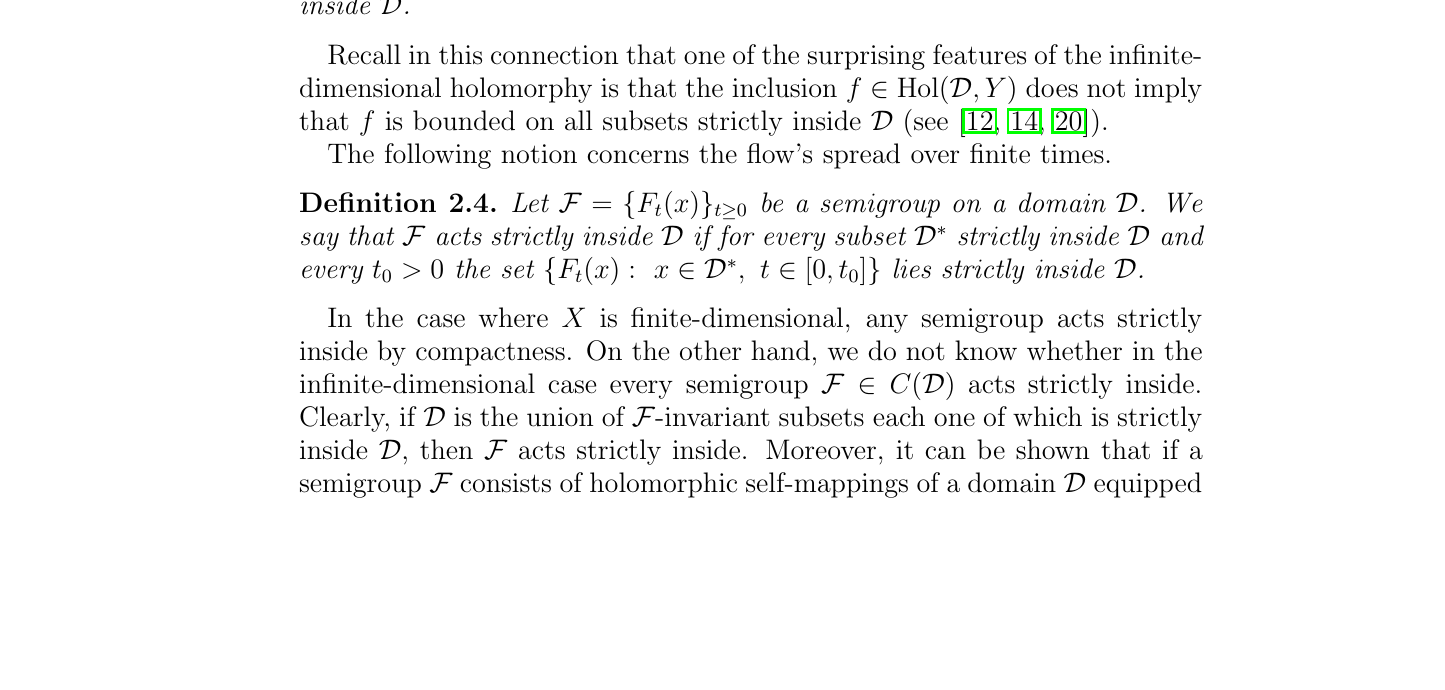
\includegraphics[width=\textwidth]{figures/strict_inside_open_question.png}
\end{center}

For a family $\{G_t:\D\to Y\}_{t\geq0}$, T-continuity at $t_0$ means
\[
 \sup_{x\in S}\|G_t(x)-G_{t_0}(x)\|\longrightarrow0
 \quad(t\to t_0)
\]
for every $S$ strictly inside $\D$. Before Proposition 3.3, the authors ask
whether T-continuity of a semicocycle at $t_0=0$ implies T-continuity for all
$t_0\geq0$. Their Proposition 3.3(ii) proves this under two extra assumptions:
the base semigroup acts strictly inside and every semicocycle map is bounded on
sets strictly inside. The open statement appears on source PDF page 10:

\begin{center}
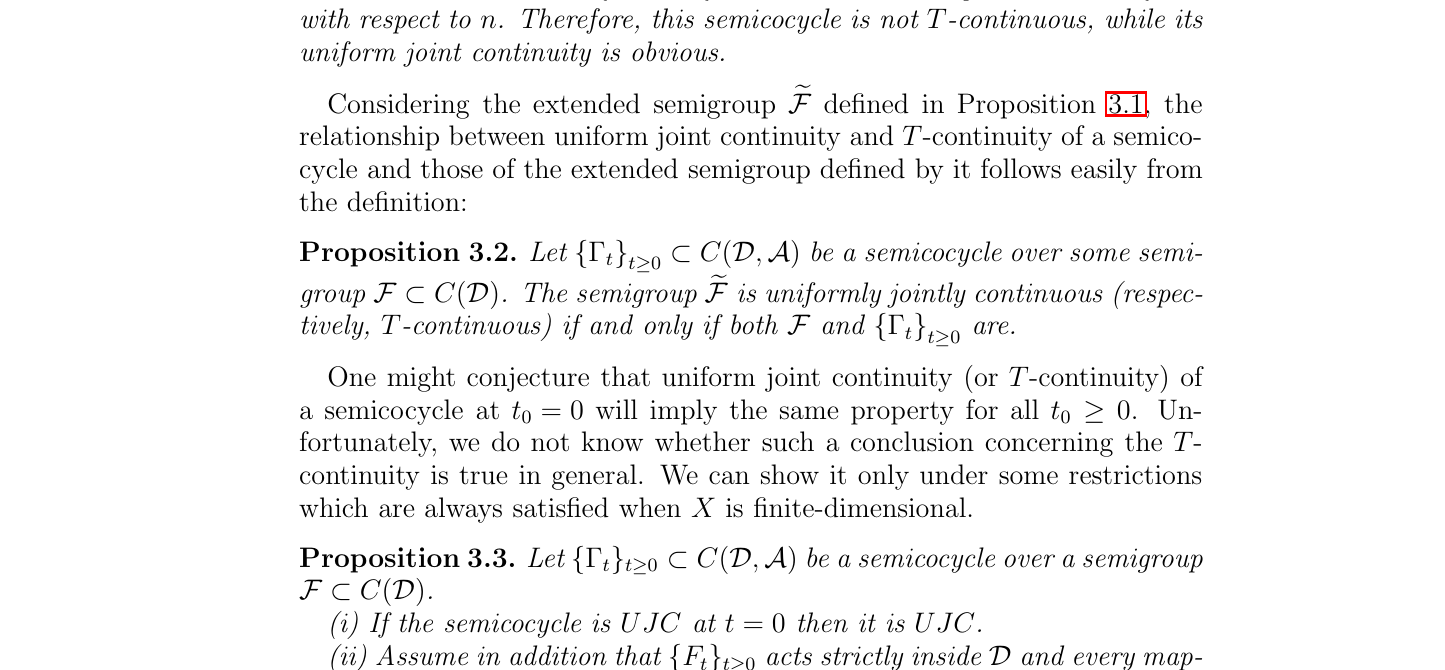
\includegraphics[width=\textwidth]{figures/t_continuity_open_question.png}
\end{center}

\section{Proof intuition}

Infinite dimension allows a smooth function to be unbounded even on a set that
stays a fixed positive distance from the boundary. We build such a function
$g$ explicitly on $\ell_2$, with $g(\frac12e_n)=n$. For each fixed $u$, the
vertical slice of the Hilbert ball is an interval. The change of coordinate
$\sigma=R(u)\tanh y$ identifies that interval with the whole real line. We let
the semigroup translate $y$ at speed $g(u)$. The basis points are therefore
sent arbitrarily close to the boundary by time one, although they began deep
inside the ball.

For the second question, a bounded coboundary
$\Gamma_t=\exp(q\circ F_t-q)$ automatically obeys the semicocycle identity.
Choose $q$ to be a smooth step whose threshold is tuned to the time-one
translation. On any fixed strictly-inside set, small-time motion is uniformly
invisible: either the speed is bounded, or both sides of the step remain in its
flat zero region. At time one, however, all basis points sit exactly at the
threshold, and an arbitrarily small further time activates a sufficiently fast
coordinate. This destroys T-continuity at time one while keeping every
$\Gamma_t$ globally bounded.

\section{An analytic speed unbounded on an interior sequence}

Let $H=\ell_2(\R)$ with standard basis $(e_k)_{k\geq1}$ and define
\begin{equation}\label{eq:g}
 g(u)=\sum_{k=1}^{\infty} k(2u_k)^{2k},\qquad u=(u_k)\in H.
\end{equation}

\begin{lemma}\label{lem:g}
The series in \eqref{eq:g} defines a nonnegative real-analytic function on
$H$. Moreover,
\[
 g\!\left(\tfrac12e_n\right)=n\qquad(n\geq1).
\]
\end{lemma}

\begin{proof}
Fix $u\in H$. Since $u_k\to0$, choose $N$ and $q_0<1$ so that
$2|u_k|\leq q_0$ for $k>N$. Choose $\delta>0$ with
$q:=q_0+2\delta<1$. If $\|v-u\|_2<\delta$, then for $k>N$,
\[
 2|v_k|\leq2|u_k|+2\|v-u\|_2<q.
\]
Hence the tail of \eqref{eq:g} is uniformly dominated on that neighborhood by
$\sum_{k>N}kq^{2k}<\infty$. The identical estimate holds for complex
$v\in\ell_2(\C)$ near the real point $u$. Thus the coordinate polynomials
$k(2v_k)^{2k}$ converge locally uniformly to a holomorphic function on the
complexification. Its restriction to $H$ is real analytic. Nonnegativity is
clear, and at $u=\frac12e_n$ only the $n$th summand is nonzero, with value
$n$.
\end{proof}

\section{The two counterexamples}

Let
\[
 X=H\oplus_2\R,\qquad
 \D=B_X=\{(u,\sigma):\|u\|_2^2+\sigma^2<1\}.
\]
For $\|u\|_2<1$, put
\[
 R(u)=\sqrt{1-\|u\|_2^2},
 \qquad
 y(u,\sigma)=\operatorname{artanh}\!\left(\frac{\sigma}{R(u)}\right).
\]
Thus $|\sigma|<R(u)$, and $\sigma\mapsto y(u,\sigma)$ is a real-analytic
diffeomorphism from the vertical slice $(-R(u),R(u))$ onto $\R$.

For $t\geq0$, define
\begin{equation}\label{eq:F}
 F_t(u,\sigma)=
 \left(u,R(u)\tanh\bigl(y(u,\sigma)+t g(u)\bigr)\right).
\end{equation}

Choose a $C^\infty$ nondecreasing function $Q:\R\to[0,1]$ satisfying
\begin{equation}\label{eq:Q}
 Q(r)=0\ (r\leq0),\qquad Q(r)=1\ (r\geq1).
\end{equation}
For example, one may use the standard transition constructed from
$\theta(r)=0$ for $r\leq0$ and $\theta(r)=e^{-1/r}$ for $r>0$:
$Q(r)=\theta(r)/(\theta(r)+\theta(1-r))$. Set
\begin{equation}\label{eq:qGamma}
 q(u,\sigma)=Q\bigl(y(u,\sigma)-g(u)\bigr),
 \qquad
 \Gamma_t(x)=\exp\bigl(q(F_t(x))-q(x)\bigr).
\end{equation}

\begin{theorem}\label{thm:main}
The following assertions hold.
\begin{enumerate}
\item The family $\F=\{F_t\}_{t\geq0}$ is a semigroup of real-analytic
self-maps of the open unit ball of an infinite-dimensional real Hilbert space,
but $\F$ does not act strictly inside $\D$.
\item With the unital complex Banach algebra $\mathcal A=\C$, the family
$\{\Gamma_t\}_{t\geq0}$ is a globally bounded $C^\infty$ scalar semicocycle
over $\F$. It is T-continuous at $t=0$ but is not T-continuous at $t=1$.
In fact $e^{-1}\leq\Gamma_t(x)\leq e$ for every $t\geq0$ and $x\in\D$.
\end{enumerate}
Consequently, both general questions above have negative answers.
\end{theorem}

\begin{proof}
Because $|\tanh r|<1$ for real $r$, formula \eqref{eq:F} maps $\D$ into
$\D$. It is real analytic by Lemma~\ref{lem:g}. In the $y$ coordinate it is
simply
\[
 (u,y)\longmapsto (u,y+t g(u)).
\]
Therefore $F_0$ is the identity and $F_t\circ F_s=F_{t+s}$. Also
$F_t(x)\to x$ as $t\to0^+$ for every $x$, so $\F$ is a continuous semigroup
in the precise sense used in~\cite{EJK}.

Now put
\[
 p_n=\left(\tfrac12e_n,0\right)\in\D.
\]
Every $p_n$ has norm $1/2$. Thus $P=\{p_n:n\geq1\}$ is bounded and
$\dist(P,\partial\D)=1/2$, so $P$ lies strictly inside $\D$. At $p_n$ we have
$R(\frac12e_n)=\sqrt3/2$, $y(p_n)=0$, and $g(\frac12e_n)=n$. Consequently,
\[
 F_1(p_n)=
 \left(\tfrac12e_n,\tfrac{\sqrt3}{2}\tanh n\right),
 \qquad
 \|F_1(p_n)\|^2=\frac14+\frac34\tanh^2 n\longrightarrow1.
\]
Thus $\inf_n\dist(F_1(p_n),\partial\D)=0$. The finite-time orbit set for
$P$ and $t_0=1$ is not strictly inside $\D$, proving part~1.

The function $q$ is smooth and $0\leq q\leq1$. The coboundary formula gives
$\Gamma_0=1$, and for $s,t\geq0$,
\begin{align*}
 \Gamma_t(F_sx)\Gamma_s(x)
 &=\exp\bigl(q(F_tF_sx)-q(F_sx)+q(F_sx)-q(x)\bigr)\\
 &=\Gamma_{t+s}(x).
\end{align*}
Pointwise time continuity follows from that of $F_t$, so this is a smooth
scalar semicocycle in the source sense. Since $q(F_t x)-q(x)\in[-1,1]$,
$e^{-1}\leq\Gamma_t(x)\leq e$ globally.

It remains to prove the two time-continuity claims. Let $S$ be any subset
strictly inside the unit ball. There is $r<1$ such that $\|x\|\leq r$ for all
$x=(u,\sigma)\in S$. Writing $a=\|u\|_2^2$, we have
\[
 \left|\frac{\sigma}{R(u)}\right|^2
 \leq\frac{r^2-a}{1-a}\leq r^2.
\]
Hence
\begin{equation}\label{eq:ybound}
 |y(x)|\leq M:=\operatorname{artanh}r\qquad(x\in S).
\end{equation}
Let $L=\|Q'\|_\infty$. Since $F_h$ adds $h g(u)$ to $y$,
\begin{equation}\label{eq:loggamma}
 \log\Gamma_h(u,\sigma)
 =Q\bigl(y-(1-h)g(u)\bigr)-Q\bigl(y-g(u)\bigr).
\end{equation}
For $0<h\leq1/2$, split into two cases. If $g(u)\geq2M$, both arguments in
\eqref{eq:loggamma} are at most zero, so the difference vanishes. If
$g(u)\leq2M$, the mean value theorem gives
\[
 |\log\Gamma_h(u,\sigma)|\leq Lh g(u)\leq2LMh.
\]
Thus $\log\Gamma_h\to0$, and hence $\Gamma_h\to1$, uniformly on every
strictly-inside $S$. The semicocycle is T-continuous at zero.

Finally consider the same strictly-inside set $P=\{p_n\}$. At $p_n$,
$y=0$, $g=n$, and therefore $q(p_n)=Q(-n)=0$. At time one the new $y$-value
is $n$, so $q(F_1p_n)=Q(0)=0$ and $\Gamma_1(p_n)=1$. But for every $h>0$ and
every integer $n\geq1/h$,
\[
 q(F_{1+h}p_n)=Q(hn)=1,
 \qquad
 \Gamma_{1+h}(p_n)=e.
\]
It follows that
\[
 \sup_{x\in P}|\Gamma_{1+h}(x)-\Gamma_1(x)|\geq e-1
 \qquad(h>0).
\]
Therefore T-continuity fails at $t=1$, proving part~2.
\end{proof}

\section{Consequences, limitations, and novelty check}

Part~1 directly disproves the proposed general infinite-dimensional
strict-inside property, even for a bounded convex domain in a real Hilbert
space and a real-analytic semigroup. Part~2 shows that the strict-inside
assumption in Proposition 3.3(ii) cannot simply be deleted, even when every
semicocycle map is globally bounded and all data are smooth.

The construction is deliberately real. It does not contradict the source's
observation that semigroups of holomorphic self-maps on domains equipped with
the hyperbolic metric act strictly inside. No assertion is made about a
holomorphic analogue of this example on a complex hyperbolic domain.

Before promotion, a bounded literature search was performed on 11 August 2026
over arXiv and general scholarly web indexes. Queries included the exact paper
title and arXiv id, the two quoted open-question sentences, and combinations of
``semigroup acts strictly inside'', ``infinite-dimensional Banach'', and
``T-continuity at time zero''. The search found the source paper and neighboring
literature but no later paper explicitly answering either question and no
matching counterexample. This is a bounded novelty check, not a comprehensive
priority claim.

\paragraph{Human-review recommendation.}
Review is recommended at high priority. The principal points to check are the
local uniform convergence on the complexification in Lemma~\ref{lem:g}, the
global definition of the Hilbert-ball coordinate flow, and the two-case
estimate following \eqref{eq:loggamma}.

\begin{thebibliography}{9}
\bibitem{EJK}
M. Elin, F. Jacobzon, and G. Katriel,
\emph{Continuous and holomorphic semicocycles in Banach spaces},
J. Evol. Equ. \textbf{19} (2019), 1199--1221;
arXiv:1807.09965; DOI: 10.1007/s00028-019-00509-5.
\end{thebibliography}

\end{document}
